%\documentclass[mathserif]{beamer}
\documentclass[handout]{beamer}
%\usetheme{Goettingen}
\usetheme{Warsaw}
%\usetheme{Singapore}
%\usetheme{Frankfurt}
%\usetheme{Copenhagen}
%\usetheme{Szeged}
%\usetheme{Montpellier}
%\usetheme{CambridgeUS}
%\usecolortheme{}
%\setbeamercovered{transparent}
\usepackage[english, activeacute]{babel}
\usepackage[utf8]{inputenc}
\usepackage{amsmath, amssymb}
\usepackage{dsfont}
\usepackage{graphics}
\usepackage{cases}
\usepackage{graphicx}
\usepackage{pgf}
\usepackage{epsfig}
\usepackage{amssymb}
\usepackage{multirow}	
\usepackage{amstext}
\usepackage[ruled,vlined,lined]{algorithm2e}
\usepackage{amsmath}
\usepackage{epic}
\usepackage{epsfig}
\usepackage{fontenc}
\usepackage{framed,color}
\usepackage{palatino, url, multicol}
\usepackage{listings}
%\algsetup{indent=2em}
\newcommand{\factorial}{\ensuremath{\mbox{\sc Factorial}}}
\newcommand{\BIGOP}[1]{\mathop{\mathchoice%
{\raise-0.22em\hbox{\huge $#1$}}%
{\raise-0.05em\hbox{\L
\usepackage{fontenc}
\usepackage{framed,color}
\usepackage{palatino, url, multicol}
\usepackage{listings}
%\algsetup{indent=2em}
\newcommand{\factorial}{\ensuremath{\mbox{\sc Factorial}}}
\newcommand{\BIGOP}[1]{\mathop{\mathchoice%
{\raise-0.22em\hbox{\huge $#1$}}%
{\raise-0.05em\hbox{\Large $#1$}}{\hbox{\large $#1$}}{#1}}}
\newcommand{\bigtimes}{\BIGOP{\times}}
\vspace{-0.5cm}
\title{Introduction to Statistical Inference}
\vspace{-0.5cm}
\author[Felipe Bravo Márquez]{\footnotesize
%\author{\footnotesize  
 \textcolor[rgb]{0.00,0.00,1.00}{Felipe José Bravo Márquez}} 
\date{ \today }
arge $#1$}}{\hbox{\large $#1$}}{#1}}}
\newcommand{\bigtimes}{\BIGOP{\times}}
\vspace{-0.5cm}
\title{Introduction to Bayesian Inference}
\vspace{-0.5cm}
\author[Felipe Bravo Márquez]{\footnotesize
%\author{\footnotesize  
 \textcolor[rgb]{0.00,0.00,1.00}{Felipe José Bravo Márquez}} 
\date{ \today }


\begin{document}
\begin{frame}
\titlepage


\end{frame}


%%%%%%%%%%%%%%%%%%%%%%%%%%%


\begin{frame}{Some Critics to the Frequentist Approach}
\scriptsize{
\begin{itemize}
 \item The statistical methods that we have discussed so far are known as frequentist (or classical) methods.
  \item The frequentist approach requires that all probabilities be defined by connection to the frequencies of events in very large samples. 
 \item This leads to frequentist uncertainty being premised on imaginary resampling of data. 
 \item If we were to repeat the measurement many many times, we would end up collecting a list of values that will have some pattern to it. 
 \item  It means also that parameters and models cannot have probability distributions, only measurements can.
 \item The distribution of these measurements is called a sampling distribution. 
 \item This resampling is never done, and in general it doesn't even make sense.
\end{itemize}

} 
\end{frame}

\begin{frame}{Bayesian Inference}
\scriptsize{
There is another approach to inference called Bayesian inference \cite{wasserman2013all}, which is based on the following postulates:
\begin{itemize}
 \item Probability describes \textbf{degree of belief}, not limiting frequency. 
 
 \begin{itemize}
 \scriptsize{
 \item  We can make probability statements about lots of things, not just data which are subject to random variation. 
 \item For example, I might say that "the probability that Albert Einstein drank a cup of tea on August 1, 1948" is .35. 
 \item This does not refer to any limiting frequency. 
 \item It reflects my strength of belief that the proposition is true.}
 \end{itemize}
 
 \item We can make probability statements about parameters, even though they are fixed constants.
 \item We make inferences about a parameter $\theta$ by producing a probability distribution for $\theta$. Inferences, such as point estimates and interval estimates, may then be extracted from this distribution.
\end{itemize}

} 
\end{frame}


\begin{frame}{Bayesian Inference}
\scriptsize{
\begin{itemize}
 \item In modest terms, Bayesian data analysis is no more than counting the numbers of ways
the data could happen, according to our assumptions \cite{mcelreath2020statistical}.
 \item In Bayesian analysis all alternative sequences of events that could have generated our data are evaluated.
 \item As we learn about what did happen, some of these alternative sequences are pruned. 
 \item In the end, what remains is only what is logically consistent with our knowledge \cite{mcelreath2020statistical}.
 \item Warning: understanding the essence of Bayesian inference can be hard.
 \item The following toy example tries to explain it in a gentle way.
\end{itemize}
 } 
\end{frame}


\begin{frame}{Counting Possibilities}
\scriptsize{
\begin{itemize}
 \item Suppose there's a bag, and it contains four marbles.
 \item These marbles come in two colors: blue and white. 
 \item We know there are four marbles in the bag, but we don't know how many are of each color. 
 \item We do know that there are five possibilities: 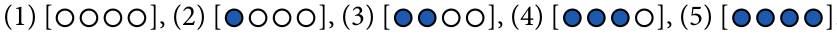
\includegraphics[scale=0.3]{pics/marbles1.png}
 \item These are the only possibilities consistent with what we know about the contents of the bag. Call these five possibilities the conjectures.
 \item Our goal is to figure out which of these conjectures is most plausible, given some evidence about the contents of the bag. 
 \item We do have some evidence: A sequence of three marbles is pulled from the bag, one at a time, replacing the marble each time and shaking the bag, in that order. These before drawing another marble.
 \item The sequence that emerges is: 
\includegraphics[scale=0.3]{pics/marbles2.png}, in that order. These are the data.
 
 
\end{itemize}
 } 
\end{frame}

%%%%%%%%%%%%%%%%%%%%%%%%%%%
\begin{frame}[allowframebreaks]\scriptsize
\frametitle{References}
\bibliography{bio}
\bibliographystyle{apalike}
%\bibliographystyle{flexbib}
\end{frame}  









%%%%%%%%%%%%%%%%%%%%%%%%%%%

\end{document}
